%!TEX TS-program = xelatex
\documentclass[a4paper, 12pt]{article}
\usepackage{barinovxesimple}
\geometry{top=25mm}
\geometry{bottom=35mm}
\geometry{left=35mm}
\geometry{right=20mm}
\setlist{labelindent=\parindent,leftmargin=*}
\begin{document}

\thispagestyle{empty}
\begin{center}
    \textit{Федеральное государственное автономное образовательное\\ учреждение высшего образования }

    \vspace{0.5ex}

        \textbf{«Московский физико-технический институт\\ (национальный исследовательский университет)»}
\end{center}

\vspace{10ex}

\begin{center}
    \vspace{13ex}

    \so{\textbf{Лабораторная работа №-.-.-}}

    \vspace{1ex}

    по курсу общей физики

    на тему:

    \textbf{\textit{<<>>}}

    \vspace{30ex}

    \begin{flushright}
        \noindent
        \textit{Работу выполнил:}\\  
        \textit{Баринов Леонид \\(группа Б02-827)}
    \end{flushright}
    \vfill
    Долгопрудный \\2019
\newpage
\setcounter{page}{1}
\fancyhead[R]{\nouppercase{\leftmark}}	
\end{center}

\section{Цель работы}
Провести исследование энергетического спектра
$\gamma$-квантов, рассеянных на графите. Определить зависимость
энергии рассеянных $\gamma$-квантов в от угла рассеяния, а также
получить энергию покоя частиц, на которых происходит комптоновское
рассеяние.



\section{Суть исследуемого явления}
\emph{Эффект Комптона} --- увеличение длины волны рассеянного
излучения по сравнению с падающим. Интерпретируется как результат
упругого соударения двух частиц: $\gamma$-кванта (фотона) и свободного
электрона.



\section{Теория явления}

\begin{wrapfigure}{r}{0.3\linewidth}
    \includegraphics[width=\linewidth]{1}
    \caption{Векторная диаграмма рассеяния $\gamma$-кванта на
    электроне}
    \label{fig:1}
\end{wrapfigure}


Пусть электрон до соударения покоился, а $\gamma$-квант имел начальную
энергию $\hbar \omega_0$ и импульс $\hbar \omega_0 /c$. После
соударения электрон приобретает энергию $\gamma m c^2$ и импульс
$\gamma m v$, где $\gamma = 1/\sqrt{1-\beta^2}$, $\beta = v/c$, а
$\gamma$-квант рассеивается на некоторый угол $\theta$ по отношению к
первоначальному направлению движения. Энергия и импульс
$\gamma$-кванта становят соответственно равными $\hbar \omega_1$ и
$\hbar \omega_1 /c$ \ffig{fig:1}. 

Запишем для рассматриваемого процесса законы сохранения энергии и
импульса:
\begin{equation*}
    \left\{
    \begin{gathered}
        mc^2 + \hbar \omega_0 = \gamma m c^2 + \hbar \omega_1\\
        \frac{\hbar \omega_0}{c} = \gamma m v \cos \phi + \frac{\hbar
        \omega_1}{c} \cos \theta\\
        \gamma m v \sin \phi = \frac{\hbar \omega_1}{c}\sin \theta
    \end{gathered}
    \right.
\end{equation*}

Решая совместно эти уравнения и переходя от частот $\omega_0$ и
$\omega_1$ к длинам волн $\lambda_0$ и $\lambda_1$, нетрудно получить,
что изменение длины волны рассеянного излучения равно
\begin{equation}
    \Delta \lambda = \lambda_1 - \lambda_0 = \frac{h}{mc} (1-\cos
    \theta) = \Lambda_\text{K} (1-\cos \theta),
    \label{eq:1}
\end{equation}
где $\lambda_0$ и $\lambda_1$ --- длины волн $\gamma$-кванта до и
после рассеяния, а величина
\[
    \Lambda_\text{K} = \frac{h}{mc} = 2,42 \cdot 10 ^{-10}\ \text{см}
\]
называется комптоновской длиной волны электрона. Из формулы
\eqref{eq:1} следует, что комптоновское смещение не зависит ни от
длины волны первичного излучения, ни от рода вещества, в котором
наблюдается рассеяние. В приведенном выводе электрон в атоме считается
свободным.

Применительно к условиям нашего опыта формулу \eqref{eq:1} следует
преобразовать от длин волн к энергии $\gamma$-квантов. Выражение будет
иметь вид:
\begin{equation}
    \frac{1}{\epsilon (\theta)} - \frac{1}{\epsilon_0} = 1 - \cos
    \theta
    \label{eq:2}
\end{equation}

Здесь $\epsilon_0 = E_0/ (mc^2)$--- выраженная в единицах $mc^2$
энергия $\gamma$-квантов, падающих на рассеиватель, $\epsilon(\theta)$
--- выраженная в тех же единицах энергия квантов, испытавших
комптоновское рассеяние на угол $\theta, m$ --- масса электрона.







\section{Эксперимент}
\subsection{Экспериментальная установка}
Блок-схема установки изображена на \fig{fig:2}. Источником излучения
\textsl{1} служит $ ^{137}$Cs, испускающий $\gamma$-лучи с энергией
$662\ \text{кэВ}$. Он помещен в толстостенный свинцовый контейнер с
коллиматором. Сформированный коллиматором узкий пучок $\gamma$-квантов
попадает на графитовую мишень \textsl{2} (цилиндр диаметром $40\
\text{мм}$ и высотой $100\ \text{мм}$).

\begin{figure}[H]
    \includegraphics[width=0.7\linewidth]{3} 
    \caption{Блок-схема установки по изучению рассеяния
    $\gamma$-квантов}
    \label{fig:2}
\end{figure}

Кванты, испытывающие комптоновское рассеяние в мишени, регистрируются
сцинтилляционным счетчиком. Счетчик состоит из фотоэлектронного
умножителя \textsl{3} (далее ФЭУ) и сцинтиллятора \textsl{4}. Сцинтиллятором служит
кристалл NaI(Tl) цилиндрической формы диаметром $40\: \text{мм}$ и
высотой $40\: \text{мм}$, его выходное окно находится в оптическом
контакте с фотокатодом ФЭУ. Сигналы, возникающие на аноде ФЭУ,
подаются на ЭВМ для амплитудного анализа. Кристалл и ФЭУ расположены в
светонепроницаемом блоке, укрепленном на горизонтальной штанге. Штанга
вместе с этим блоком может вращаться относительно мишени, угол
поворота отсчитывается по лимбу \textsl{6}.

Головная часть сцинтилляционного блока закрыта свинцовым коллиматором
\textsl{5}, который формирует входной пучок и защищает детектор от
постороннего излучения. Основной вклад в это излучение вносят
$\gamma$-кванты, проходящие из источника \textsl{1} через
$6$-сантиметровые стенки защитного контейнера. Этот фон особенно
заметен при исследовании комптоновского рассеяния на большие углу
$(\simeq 120 ^{\circ})$, когда расстояние между детектором и
источником уменьшается.


Существуют три механизма взаимодействия $\gamma$-квантов с веществом:
комптоновское рассеяние, фотоэффект и рождение электрон-позитронных
пар (в нашем случае этот механизм не реализуется, так как энергия
$\gamma$-квантов не превосходит порог рождения пар). Во всех этих
случаях в веществе появляется быстрый электрон, который за счет
кулоновского взаимодействия эффективно возбуждает на своем пути атомы
и молекулы.

При фотоэффекте $\gamma$-квант целиком поглащается атомом, а один из
электронов внутренней оболочки выбрасывается за пределы атома, унося
все переданную $\gamma$-квантом энергию и теряя ее затем в кристалле.
При комптоновском рассеянии электрону передается только часть энергии
$\gamma$-кванта, а оставшаяся часть уносится рассеянным
$\gamma$-квантом.


\begin{wrapfigure}{l}{0.5\linewidth}
    \includegraphics[width=\linewidth]{5}
    \caption{Амплитудное распределение импульсов, возникающих под
    действием монохроматических $\gamma$-квантов в сцинтилляторе
NaI(Ti)}
\label{fig:5}
\end{wrapfigure}

Таким образом, под действием монохроматического излучения на выходе
ФЭУ возникает распределение электрических импульсов, показанное на
\fig{fig:5}. В амплитудном распределении импульсов имеется так
называемый фотопик, возникающий в результате фотоэффекта, и обязанное
комптоновскому рассеянию сплошное распределение. Его положение
однозначно связано в энергией регистрируемого $\gamma$-излучения.

Слева от фотопика после большого провала начинается непрерывный спектр
комптоновских электронов. Этот фон сохраняется при любом угле
рассеяния и мешает определению фотопика рассеянных $\gamma$-квантов.
Его положение легко идентифицируется при рассмотрении всех
зарегистрированных спектров.

Для определения энергии $\gamma$-квантов нужно исследовать кривую
распределения энергетических потерь в кристалле, т.е. распределение по
амплитуде электрических импульсов на выходе ФЭУ. Такое распределение
измеряется в данной работе с помощью компьютера, работающего в режиме
амплитудного анализатора.










\section{Результаты эксперимента}


\renewcommand{\arraystretch}{1.5}
\begin{table}[H]
\centering
\begin{tabular}{|c|c|c|c|c|c|c|c}
\hline 
$\theta, ^{\circ}$ & 0   & 10  & 20  & 30  & 40  & 50  & \multicolumn{1}{c|}{60}  \\ \hline
$N$ & 824 & 839 & 704 & 685 & 595 & 531 & \multicolumn{1}{c|}{491} \\
\hline \hline 
$\theta, ^{\circ}$ & 70  & 80  & 90  & 100 & 110 & 120 & \multirow{2}{*}{}        \\ \cline{1-7}
$N$ & 432 & 384 & 352 & 332 & 288 & 253 &                          \\ \cline{1-7}
\end{tabular}
\caption{Зависимость номера канала $N$ от угла рассеяния $\theta$}
\end{table}


Построим график зависимости величины, обратной к номеру канала $1/N$
от $(1-\cos \theta)$. 


\begin{figure}[H]
    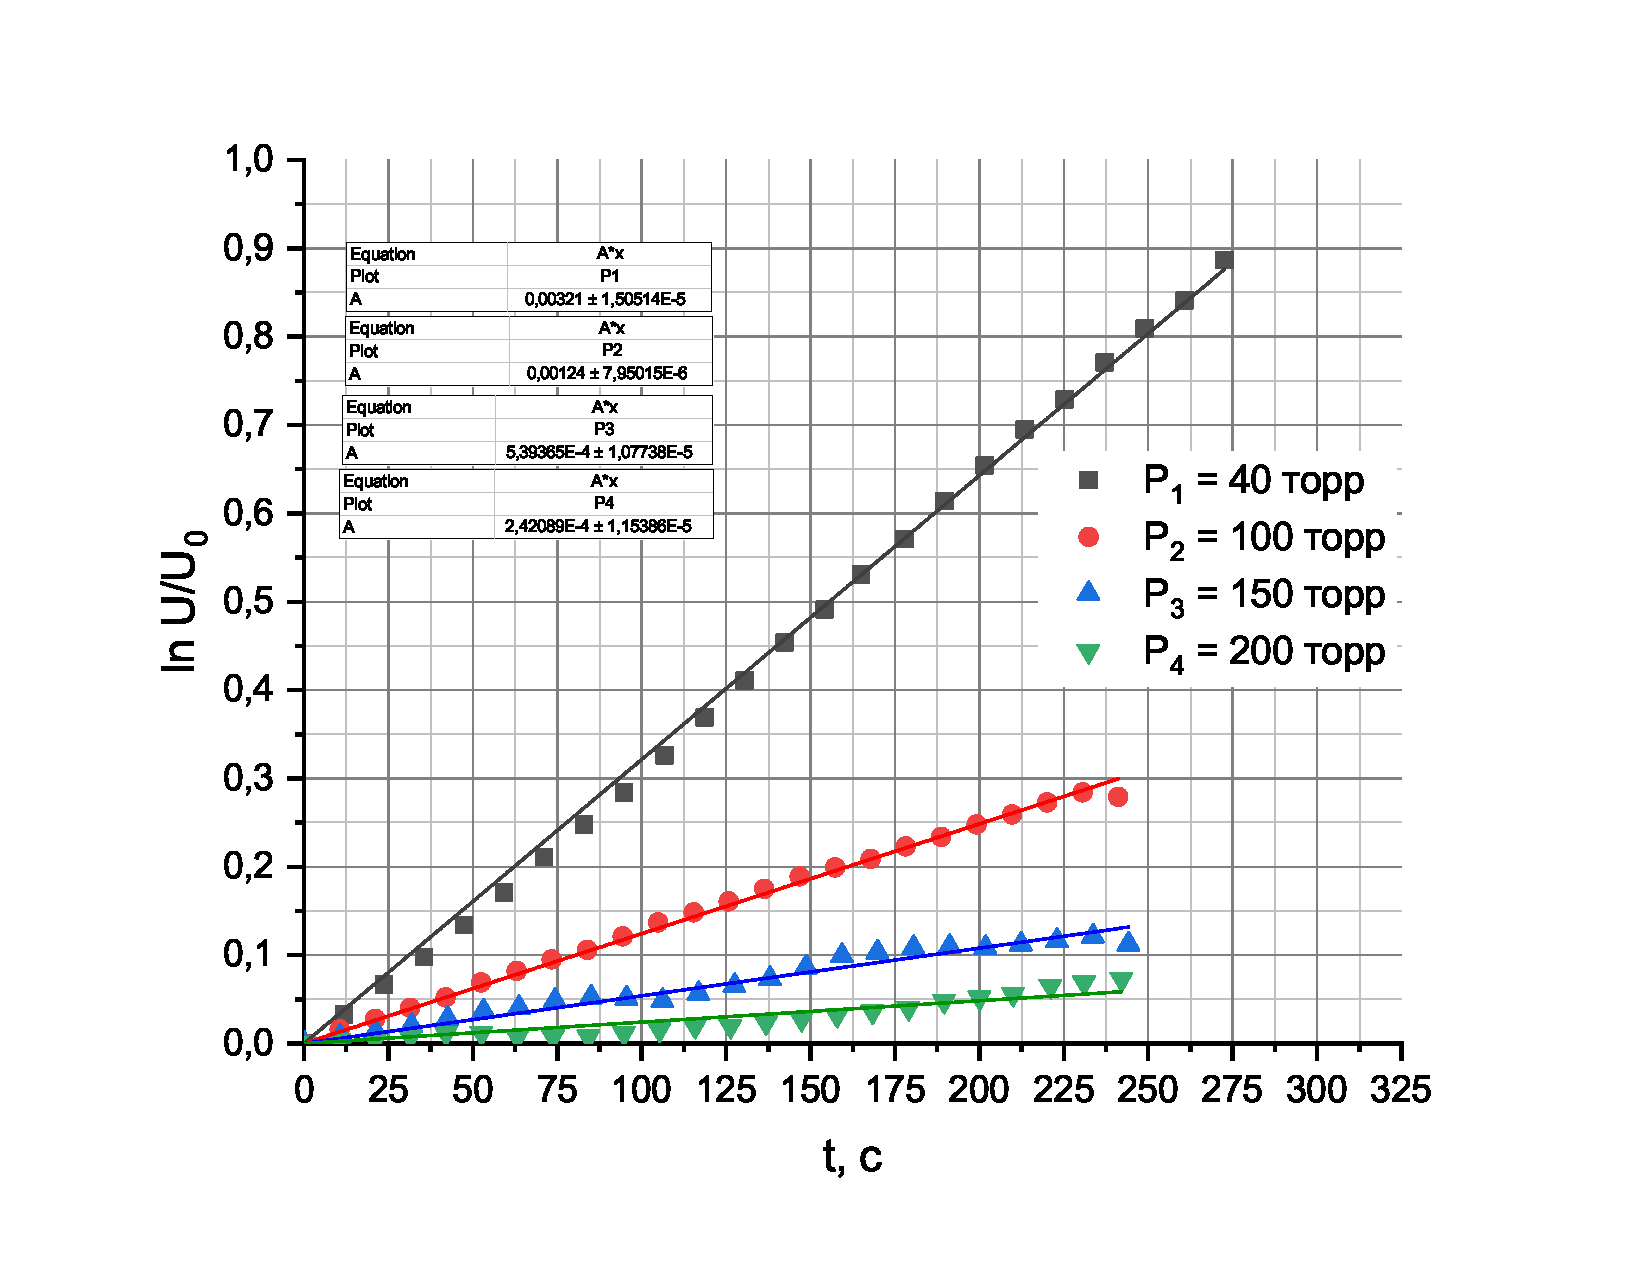
\includegraphics[width=\linewidth]{6} 
    \caption{График зависимости величины, обратной к номеру канала $1/N$
от $(1-\cos \theta)$}
\label{fig:6}
\end{figure}







\section{Анализ результатов}
Заменим в формуле \eqref{eq:2} энергию квантов, испытавших
комптоновское рассеяние на угол $\theta$, номером канала $N(\theta)$,
соответствующего вершине фотопика при указанном угле $\theta$.
Обозначая буквой $A$ неизвестный коэффициент пропорциональности между
$\epsilon (\theta)$ и $N (\theta)$, найдем:
\begin{equation}
    \frac{1}{N (\theta)} - \frac{1}{N(0)} = A (1 - \cos \theta)
    \label{eq:3}
\end{equation}


Пересечение прямой на \fig{fig:6} с осью ординат определяет наилучшее
значение $N _{\text{наил}} (0)$. 
\begin{equation*}
    \begin{gathered}
    1/N _{\text{наил}} (0) = (1,23 \pm 0,04) \cdot 10 ^{-3}\\
    N _{\text{наил}} (0) = 813 \pm 26
    \end{gathered}
\end{equation*}


Пересечение линии \ffig{fig:6} с прямой $\cos \theta = 0$ позволяет найти наилучшее
значение $N _{\text{наил}} (90)$.
\begin{equation*}
    \begin{gathered}
    1/N _{\text{наил}} (90) = (2,91 \pm 0,09) \cdot 10 ^{-3}\\
    N _{\text{наил}} (90) = 343 \pm 10
    \end{gathered}
\end{equation*}


Найдем энергию покоя частиц, на которых происходит комптоновское
рассеяние. Вернемся от переменной $\epsilon$ к энергии $E$ в формуле
\eqref{eq:2}. При $\theta = 90 ^{\circ}$ формула принимает вид
\begin{equation}
    mc^2 = E (0) \frac{ E (90) }{ E (0) - E (90) } = E _{\gamma}
    \frac{N (90)}{N (0) - N (90)}
    \label{eq:4}
\end{equation}

$E (0) = E _{\gamma}$ --- энергия электронов, рассеянных вперед, ---
просто равна энергии $\gamma$-лучей, испускаемых источником. 
\[
    mc^2 = (0,48 \pm 0,3)\: \text{МэВ}
\]

\section{Выводы}
В работе был исследован энергетический спектр $\gamma$-квантов,
рассеянных на графите. Была определена энергия рассеянных
$\gamma$-квантов в зависимости от угла рассеяния
\ffig{fig:6}, что подтверждает справедливость формулы
\eqref{eq:2}. Из полученной зависимости на \fig{fig:6} найдена
энергия покоя частиц, на которых происходит комптноновское
рассеяние:
\[
    mc^2 = (0,48 \pm 0,3)\: \text{МэВ}
\]

Величина в пределах погрешности совпадает с табличной энергией
покоя электрона:
\[
    (m_e c^2) ^{\text{табл}} = 0,512\: \text{МэВ}
\]

Это подтверждает гипотезу о том, что комптоновское рассеяние происходит на свободных
электронах. 

















\end{document}
